% !TeX spellcheck = en_US
% !TeX root = notes.tex
\section{Lecture 3: Bitcoin, Cryptocurrencies Blockchain Technology}
\subsection{Sybil Attack}
\begin{itemize}
	\item The Sybil attack in computer security is an attack wherein a reputation system is subverted by forging identities in peer-to-peer networks.
	\item Creates a large number of false identities in order to flood the network and take it over.
	\item Named after the subject of the book \textbf{Sybil}, a case study of a woman diagnosed with multiple personality disorder
	\item Such false identities are called \textbf{``Sybils''}, in the context of P2P systems
	\item One approach to preventing these “Sybil attacks” is to have a trusted agency certify identities.
	\item Or \textbf{``Sockpuppets''} in the context of the Internet, e.g. to manipulate public opinion
	\begin{leftbar}
		``... referred to a false identity assumed by a member of an Internet community who spoke to, or about, themselves while pretending to be another person. `The term now includes other misleading uses of online identities, such as those created to praise, defend or support a person or organization, to manipulate public opinion, or to circumvent a suspension or ban from a website''\\
		- Wikipedia
	\end{leftbar}
\end{itemize}

\subsection{Decentralized Consensus in Bitcoin}
\begin{itemize}
	\item Bitcoin achieves consensus by replacing \textbf{one node (or one IP address) one vote}, with \textbf{one CPU one vote}
	\item Bitcoin mining uses mostly ASICs and GPUs, not CPUs
	\item Consensus is achieved by a (probabilistic) majority vote, based on computing power
	\begin{itemize}
		\item Attacker needs > 50\% of combined computing power in order to cheat with high probability
		\item This is harder to achieve than controlling more than half of the nodes
		\item It's relatively easy to spin up a few thousand VMs as nodes, compared to controlling >50\% of Bitcoin's mining compute power
	\end{itemize}
	\item Bitcoin combines a \textbf{proof-of-work mechanism} (based on Hashcash), combined with a clever incentive mechanism $\rightarrow$ Nodes get paid to do the right thing, i.e. checking and confirming valid transactions via ``mining''
\end{itemize}

\section{Lecture 3: Bitcoin}
\begin{itemize}
	\item Complete transaction history is stored in public ledger (blockchain), stored by nodes in P2P network
	\item New transactions are created off-line, and then broadcast is P2P network
	\item Nodes validate and relay transactions (if valid)
	\item Nodes add new transactions (not part of blockchain yet) to a \textbf{transaction pool}
	\item Nodes combine transactions in pool to a block, and try to solve the corresponding proof-of-work puzzle, to ``confirm'' the block
	\item Node that finds solution first broadcasts block with solution in the network (Winning node selection is probabilistic, with probability propertional to computing power)
	\item Nodes check solution, and if OK, add new block to their local copy of blockchain
	\item All nodes who were working on solving the old puzzle, immediately start working on a new block
	\begin{itemize}
		\item Everybody always works on the longest chain
		\item Convergence to longest chain provides consensus
		\item Forks happen but are resolved by (computational) majority vote
	\end{itemize}
\end{itemize}
\begin{note}{Bitcoin Components}
	\begin{itemize}
		\item Bitcoin Network
		\item Bitcoin Identities/Addresses
		\item Bitcoin Transactions
		\item Bitcoin Scripting Language
		\item Blocks
		\item Proof-of-work, Hash puzzles, Mining
		\item Consensus
	\end{itemize}
\end{note}

\subsection{Bitcoin Network}
Transactions are broadcast in the Bitcoin network, consisting of ``full'' Bitcoin nodes ($\approx$10,000)
\begin{itemize}
	\item Best-effort (asynchronous, unreliable), it's enough if only some nodes get the message
	\item It's easy to join the Bitcoin Network, just download and run the client (Bitcoin is a \textbf{permissionless, public} blockchain, anyone can join)
\end{itemize}
Network is unstructured P2P network (random topology)
\begin{itemize}
	\item Similar to Gnutella (a P2P system from a long time ago)
	\item Overlay network, TCP, port 8333
	\item Messages are flooded
	\item All nodes are equal, no hierarchy
	\item Nodes can join at any time
	\item Node is `forgotten' if it does not respond for more than 3 hours
	\item Network is very simple and robust, e.g. to churn, but not very efficient
\end{itemize}
\begin{note}{Bitcoin Network Nodes}
	\begin{itemize}
		\item Check validity of transactions
		\item Relay transactions in the network via flooding
		\item Mining (proof-of-work puzzles)
		\item Validate and forward confirmed blocks (Add them to local copy of blockchain)
	\end{itemize}
\end{note}
\subsection{Bitcoin Identity and Addresses}
Users are represented by their Public Key addresses (hash), called \textbf{Bitcoin Addresses}, which serve as a pseudonyms
\begin{itemize}
	\item An address is a \textbf{160 bit} value, and is computed as follows
	\item RIPEMD160 hash of SHA-256 hash of ECDSA Public Key
	\item This is a ``Pay-to-pubkey-hash (P2PKH)'' address, encoding starts with ``1''
\end{itemize}
When spending a coin, spender needs to proof ownership of coin by providing a valid digital signature on the spend transaction (i.e. proving ownership of corresponding private key)\\
How can digital signatures be verified?
\begin{itemize}
	\item We need public key, not just hash of public key
	\item Spender of coin needs to provide both valid signature AND public key
	\item How do we know the provided public key is authentic $\rightarrow$ Hash it, and compare with Bitcoin address, which is the hash of public key
\end{itemize}
Bitcoin also supports \textbf{Pay to script hash (P2SH)} addresses
\begin{itemize}
	\item Allow transactions to be sent to a \textbf{script hash} instead of a public key hash (Address encoding starts with a `3' instead of `1')
	\item To spend bitcoins sent via P2SH, the recipient must provide a script matching the script hash and data which makes the script evaluate to true
	\item Allows more complex transactions (\textbf{smart contracts}), e.g. transaction outputs that require multiple signatures (multisig), or transaction puzzle, ...
\end{itemize}
\begin{note}{Bitcoin Address Encoding}
	Bitcoin uses Base58 encoding (binary-to-text encoding). Similar to Base64 encoding, but without some characters. Rationale, as explained in original bitcoin client source code:
	\begin{code}
		// Why base-58 instead of standard base-64 encoding?\\
		// - Don't want 0OIL characters that look like the same in some fonts and\\
		//   could be used to create visually identical looking account numbers.\\
		// - A string with non-alphanumeric characters is not as easily accepted as an account nbr.\\
		// - E-mail usually won't line-break if there's no punctuation to break at.\\
		// - Doubleclicking selects the whole number as one word if it's all\\alphanumeric.
	\end{code}
	Bitcoin also adds 4 byte checksum to addresses
\end{note}
\subsubsection{Bitcoin Address -- Balance}
\begin{itemize}
	\item The ``balance'' of an address is the total of unspent transaction outputs (UTXO) sent to the address.
	\item ``There are no accounts or balances in bitcoin; there are only unspent transaction outputs (UTXO) scattered in the blockchain''
	\item A user typically has many different addresses, all managed by the ``wallet'' software
	\item The wallet ``balance'' is the sum of all unspent transaction outputs of all addresses owned by the user
\end{itemize}
\subsection{Bitcoin Transactions}
\begin{itemize}
	\item Transaction are created off-line (No need to be connected to Bitcoin network for this)
	\item Transactions are broadcast in Bitcoin P2P network
	\item Nodes check validity, and relay transaction (flooding)
	\item Nodes add to new transactions to a block and try to solve hash puzzle
	\item A block with a solved puzzle is ``confirmed'', and broadcast in the network, and added to the blockchain of each node
	\item Contains:
	\begin{itemize}
		\item Inputs (any number $\geq0$)
		\item Outputs (any number > 0)
		\item Digital signatures of input coin owners (Typically for \textbf{P2PKH} transactions)
		\item Input needs to be completely consumed (With exception of Transaction Fee)
	\end{itemize}
\end{itemize}
\subsubsection{Basic Transaction Types}
\begin{itemize}
	\item Common Transaction
	\begin{itemize}
		\item 1 input
		\item 1 ``normal'' output
		\item 1 change output (back to owner)
		\subitem Create new ``Change Address'' to maintain ``anonymity''
	\end{itemize}
	\item Aggregating Transaction
	\begin{itemize}
		\item Multiple inputs
		\item 1 output
	\end{itemize}
	\item Distributing Transaction
	\begin{itemize}
		\item 1 input
		\item Multiple outputs
	\end{itemize}
	\item ``Coinbase Transaction''
	\begin{itemize}
		\item 0 input, 1 outputs
		\item Freshly created (``minted'') coins
		\item Miner gets this as a reward for solving Hash puzzle (and thereby confirming block)
		\item First transaction in every block
	\end{itemize}
\end{itemize}

\subsection{Bitcoin Scripts}
\begin{itemize}
	\item Two types of Bitcoin scripts to validate transactions
	\begin{itemize}
		\item a locking script (Typically \textbf{ScriptPubKey})
		\item and an unlocking script (Typically \textbf{ScriptSig})
	\end{itemize}
	\item A locking script is a condition placed on an output
	\item It specifies the conditions that must be met to spend or consume the output in the future
	\begin{itemize}
		\item Typically a \textbf{valid digital signature} of the claimed owner
		\item Can be other things, to implement basic `smart contracts'
	\end{itemize}
\end{itemize}
\subsubsection{Bitcoin Scripting Language ``Script''}
\begin{itemize}
	\item Allows to program conditions required for the spending of Bitcoins (``Programmable Money'')
	\item \textbf{Script} is a simple, stack based language
	\item Not Turing complete (e.g. no loops)
	\item Scripts are guaranteed to terminate after a fixed number of steps, e.g. no infinite loops
	\item Why is this a good thing?
	\begin{itemize}
		\item Avoids potential denial of service attacks on nodes, ``logic bombs''
		\item Remember: Every node runs all scripts to validate all transactions (BTW, this severely limits scalability of Bitcoin)
	\end{itemize}
	\item In contrast, Ethereum has a Turing complete scripting language
	\subitem Solves DoS attack problem by putting a price on script computation (`Gas')
\end{itemize}

\subsection{Blocks}
\begin{itemize}
	\item Transactions are grouped into blocks
	\subitem This is an optimization. Confirming individual transactions and adding them to the blockchain would be possible, but very inefficient
	\item Transactions are stored in a Merkle Tree, with the Merkle Root (Tx\_Root) stored in the block header
	\item Once confirmed (via solving hash puzzle), a block is added to the blockchain
	\item The `Nonce' is the solution of the hash puzzle
\end{itemize}
\begin{figure}[H]
	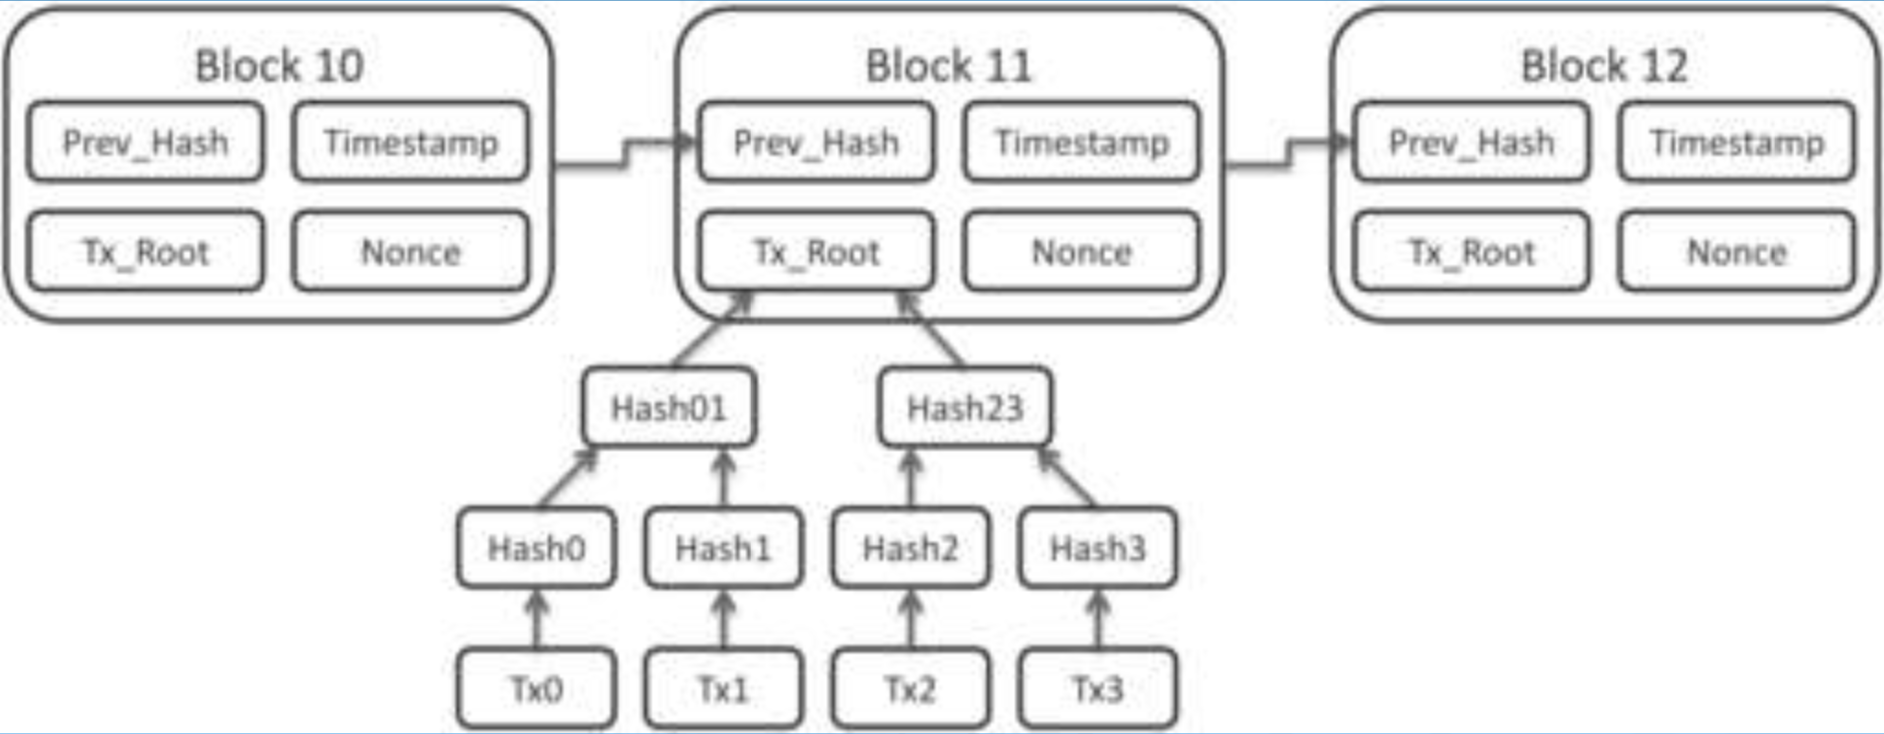
\includegraphics[width=\linewidth]{blockStructure}
	\centering
	\caption{Block Structure}
\end{figure}
\subsubsection{How are blocks added to the Blockchain?}
\begin{itemize}
	\item Multiple nodes (miners) are working towards solving the hash puzzle for a new block
	\subitem miners are probably working on different version of blocks, depending on content on their transaction pool
	\item First node who solves puzzle, broadcasts new block with solution (nonce) in the Bitcoin P2P network
	\begin{itemize}
		\item Choice of winning node is random (probabilistic)
		\item Probability of success is proportional to computing power of miner
	\end{itemize}
	\item ``Block Height'' is sequence number of blocks
	\item Other nodes check if solution is correct, and if so, add block to their local copy of the blockchain, and forward new block to other nodes
\end{itemize}

\subsection{Bitcoin Mining}
\begin{itemize}
	\item At the current level of difficulty, solving Bitcoin hash puzzles is hard and expensive
	\item Mostly ASICs based, some GPUs
	\item Total hash rate of entire Bitcoin network $\approx25\times10^{18}$H/s
	\item Hash rate of an Intel i7 CPU $\approx10$MH/s
	\subitem Need > 10,000,000 laptops to be able to mine one block per year on average
	\item Finite amount of BTC $\approx$21 Million
	\item Bitcoin is deflationary (value increases, people are potentially hoarding Bitcoin)
\end{itemize}
\subsubsection{Mining Incentive/Reward}
\begin{itemize}
	\item Transaction Fees
	\begin{itemize}
		\item Difference between total input and total output value of transaction
		\item Optional, but miners prioritize inclusion of transactions into blocks based on fees (Like giving a tip)
	\end{itemize}
	\item Block Reward
	\begin{itemize}
		\item For each solved puzzle (confirmation of block), miner currently gets freshly minted 12.5 BTC
		\item ``Coinbase transaction'' ($1^{st}$ transaction in each block)
		\item This is the only way in which coins are generated in Bitcoin
		\item Reward halved every 4 years (initially 50 BTC)
		\item Essentially no more Block Reward in 2040
	\end{itemize}
\end{itemize}

\subsection{Consensus}
\begin{itemize}
	\item Blockchain forks can happen, e.g. due to race conditions and variable latency in Bitcoin network (\textit{two nodes might find a solution to the puzzle at almost the same time}), or due to double spend attempt
	\item Nodes converge on one chain, they all aim to work on the longest (main) chain, and eventually one chain wins
	\item Incentive to work on the longest chain (Block Reward and TX fees can only be spent if block remains in the longest chain (need a certain number of \textbf{confirmations}, i.e. blocks added))
	\item Block on discontinued branches are called ``orphaned blocks''
	\item Heuristic
	\subitem Transactions are considered ``confirmed'' if they are in a block that has at least 6 blocks added to the chain (i.e. 6 confirmation) \textit{(There is nothing special about the number 6)}
	\item This means if someone wanted to reverse a transaction, they would have to go back 6 blocks, and re-do all the hash puzzles, before another nodes adds a new block at the end of chain (Practically impossible, unless attacker hash more than 50\% of computing power of entire network)
	\item Other types of attacks:
	\begin{itemize}
		\item Publish an invalid transaction, e.g. trying to spend coins that he does not own (no valid signature). Honest nodes would reject the transaction
		\item Double spend attack. Cause a fork in the chain, majority vote will guarantee that only one chain will exist
		\item Launch DoS attack against
	\end{itemize}
	\item With more than 50\% computing power, more beneficial to play by the rules and gain Block Rewards
\end{itemize}